
\documentclass[a4paper,11.5pt]{article}
\usepackage[textwidth=170mm, textheight=230mm, inner=20mm, top=20mm, bottom=30mm]{geometry}
\usepackage[normalem]{ulem}
\usepackage[utf8]{inputenc}
\usepackage[T1]{fontenc}
\PassOptionsToPackage{defaults=hu-min}{magyar.ldf}
\usepackage{pgfplots}
\pgfplotsset{compat=1.10}
\usepgfplotslibrary{fillbetween}
\usepackage[magyar]{babel}
\usepackage{amsmath, amsthm,amssymb,paralist,array, ellipsis, graphicx, float, bigints,tikz}
%\usepackage{marvosym}

\makeatletter
\renewcommand*{\mathellipsis}{%
	\mathinner{%
		\kern\ellipsisbeforegap%
		{\ldotp}\kern\ellipsisgap
		{\ldotp}\kern\ellipsisgap%
		{\ldotp}\kern\ellipsisaftergap%
	}%
}
\renewcommand*{\dotsb@}{%
	\mathinner{%
		\kern\ellipsisbeforegap%
		{\cdotp}\kern\ellipsisgap%
		{\cdotp}\kern\ellipsisgap%
		{\cdotp}\kern\ellipsisaftergap%
	}%
}
\renewcommand*{\@cdots}{%
	\mathinner{%
		\kern\ellipsisbeforegap%
		{\cdotp}\kern\ellipsisgap%
		{\cdotp}\kern\ellipsisgap%
		{\cdotp}\kern\ellipsisaftergap%
	}%
}
\renewcommand*{\ellipsis@default}{%
	\ellipsis@before
	\kern\ellipsisbeforegap
	.\kern\ellipsisgap
	.\kern\ellipsisgap
	.\kern\ellipsisgap
	\ellipsis@after\relax}
\renewcommand*{\ellipsis@centered}{%
	\ellipsis@before
	\kern\ellipsisbeforegap
	.\kern\ellipsisgap
	.\kern\ellipsisgap
	.\kern\ellipsisaftergap
	\ellipsis@after\relax}
\AtBeginDocument{%
	\DeclareRobustCommand*{\dots}{%
		\ifmmode\@xp\mdots@\else\@xp\textellipsis\fi}}
\def\ellipsisgap{.1em}
\def\ellipsisbeforegap{.05em}
\def\ellipsisaftergap{.05em}
\makeatother

\usepackage{hyperref}
\hypersetup{
	colorlinks = true	
}

\DeclareMathOperator{\Int}{int}
\DeclareMathOperator{\tg}{tg}
\DeclareMathOperator{\ctg}{ctg}
\DeclareMathOperator{\sign}{sign}
\DeclareMathOperator{\Th}{th}
\DeclareMathOperator{\sh}{sh}
\DeclareMathOperator{\ch}{ch}
\DeclareMathOperator{\arsh}{arsh}
\DeclareMathOperator{\arch}{arch}
\DeclareMathOperator{\arth}{arth}
\DeclareMathOperator{\arcth}{arcth}
\DeclareMathOperator{\grad}{grad}
\DeclareMathOperator{\arc}{arc}
\DeclareMathOperator{\arctg}{arc tg}
\DeclareMathOperator{\arcctg}{arc ctg}
\newcommand{\norm}[1]{\left\lVert#1\right\rVert}

\begin{document}
	%%%%%%%%%%%RÖVIDÍTÉSEK%%%%%%%%%%
	\setlength\parindent{0pt}
	\def\a{\textbf{a}}
	\def\b{\textbf{b}}
	\def\N{\hskip 10 true mm}
	\def\a{\textbf{a}}
	\def\b{\textbf{b}}
	\def\c{\textbf{c}}
	\def\d{\textbf{d}}
	\def\e{\textbf{e}}
	\def\gg{$\gamma$}
	\def\vi{\textbf{i}}
	\def\jj{\textbf{j}}
	\def\kk{\textbf{k}}
	\def\fh{\overrightarrow}
	\def\l{\lambda}
	\def\m{\mu}
	\def\v{\textbf{v}}
	\def\0{\textbf{0}}
	\def\s{\hspace{0.2mm}\vphantom{\beta}}
	\def\Z{\mathbb{Z}}
	\def\Q{\mathbb{Q}}
	\def\R{\mathbb{R}}
	\def\C{\mathbb{C}}
	\def\N{\mathbb{N}}
	\def\Rn{\mathbb{R}^{n}}
	\def\Ra{\overline{\mathbb{R}}}
	\def\sume{\displaystyle\sum_{n=1}^{+\infty}}
	\def\sumn{\displaystyle\sum_{n=0}^{+\infty}}
	\def\biz{\emph{Bizonyítás:\ }}
	\def\narrow{\underset{n\rightarrow+\infty}{\longrightarrow}}
	\def\limn{\displaystyle\lim_{n\to +\infty}}
	%	\def\definition{\textbf{Definíció:\ }}
	%	\def\theorem{\textbf{Tétel:\ }}
	%\def\note{\emph{Megjegyzés:\ }}
	%\def\example{\textbf{Példa:\ }} 
	
	\theoremstyle{definition}
	\newtheorem{theorem}{Tétel}[subsubsection]
	
	\theoremstyle{definition}
	\newtheorem{definition}[theorem]{Definíció}
	\newtheorem{example}[theorem]{Példa}
	\newtheorem{exercise}[theorem]{Házi feladat}
	\newtheorem{note}[theorem]{Megjegyzés}
	\newtheorem{task}[theorem]{Feladat}
	\newtheorem{revision}[theorem]{Emlékeztető}
	%%%%%%%%%%%%%%%%%%%%%%%%%%%%%%%%%
	\begin{center}
		{\LARGE\textbf{Az analízis alkalmazásai}}
		\smallskip

		{\Large Gyakorlati jegyzet}

		\smallskip
		3. óra.
	\end{center}
	A jegyzetet \textsc{Umann} Kristóf készítette \textsc{Kovács} Sándor gyakorlatán. (Utoljára frissítve: \today)
	\section{Helyettesítéses integrálás (folyt.)}
	\begin{task}
		$ \varOmega\subset\R^2$ tartomány: 
		$$ \varOmega:=\{x+3y=0\}\cup\{x-3y=0\}\cup\{x+3y=6\}\cup\{x-3y=6\}$$
		\begin{enumerate}
			\item Vázoljuk $ \varOmega$-t!
			\item Írjuk le $ \varOmega$-t az $u:=x+3y,\ v:=x-3y$ koordinátatrasznformációkkal!
			\item $\int_ \varOmega xy\,d(x,y)=?$
		\end{enumerate}
		
		Megoldás (1.): Megállapítható, hogy az első két egyenlet közös gyöke a (0,0), a második kettőnek a (6,0).
		\begin{figure}[h]
			\centering
			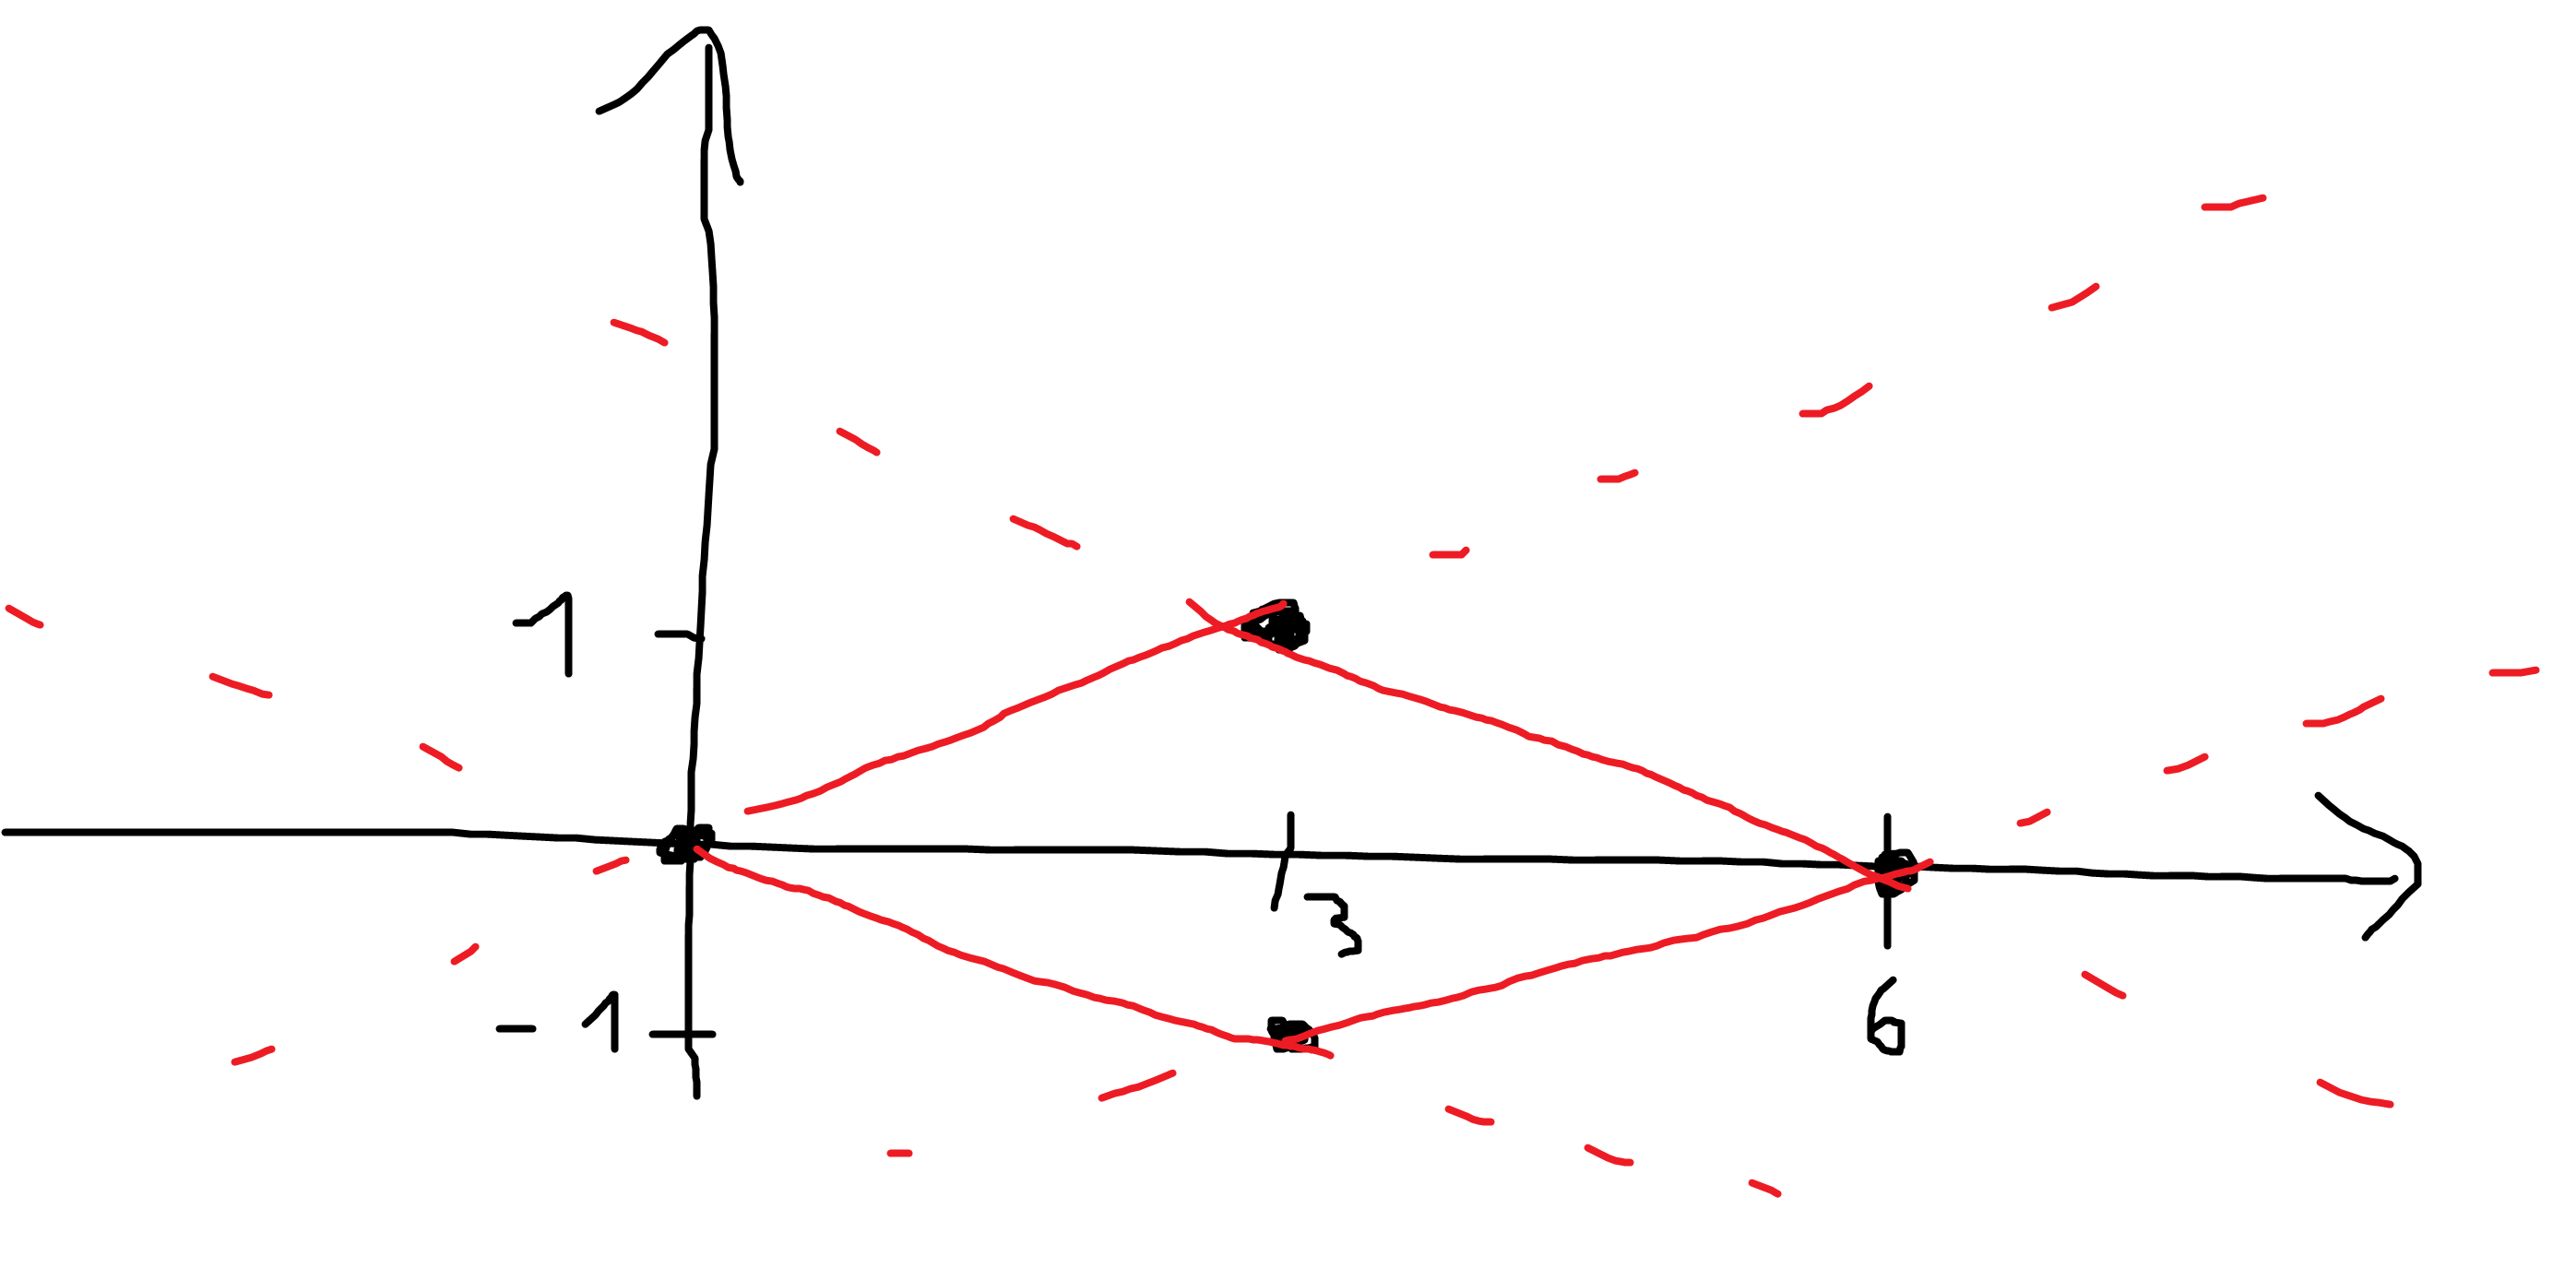
\includegraphics[width=7cm]{kepek/01.png}
			\caption{$\varOmega$ egy rombusz.}
		\end{figure}
		
		Megoldás (2.): 
		\begin{figure}[h]
			\centering
			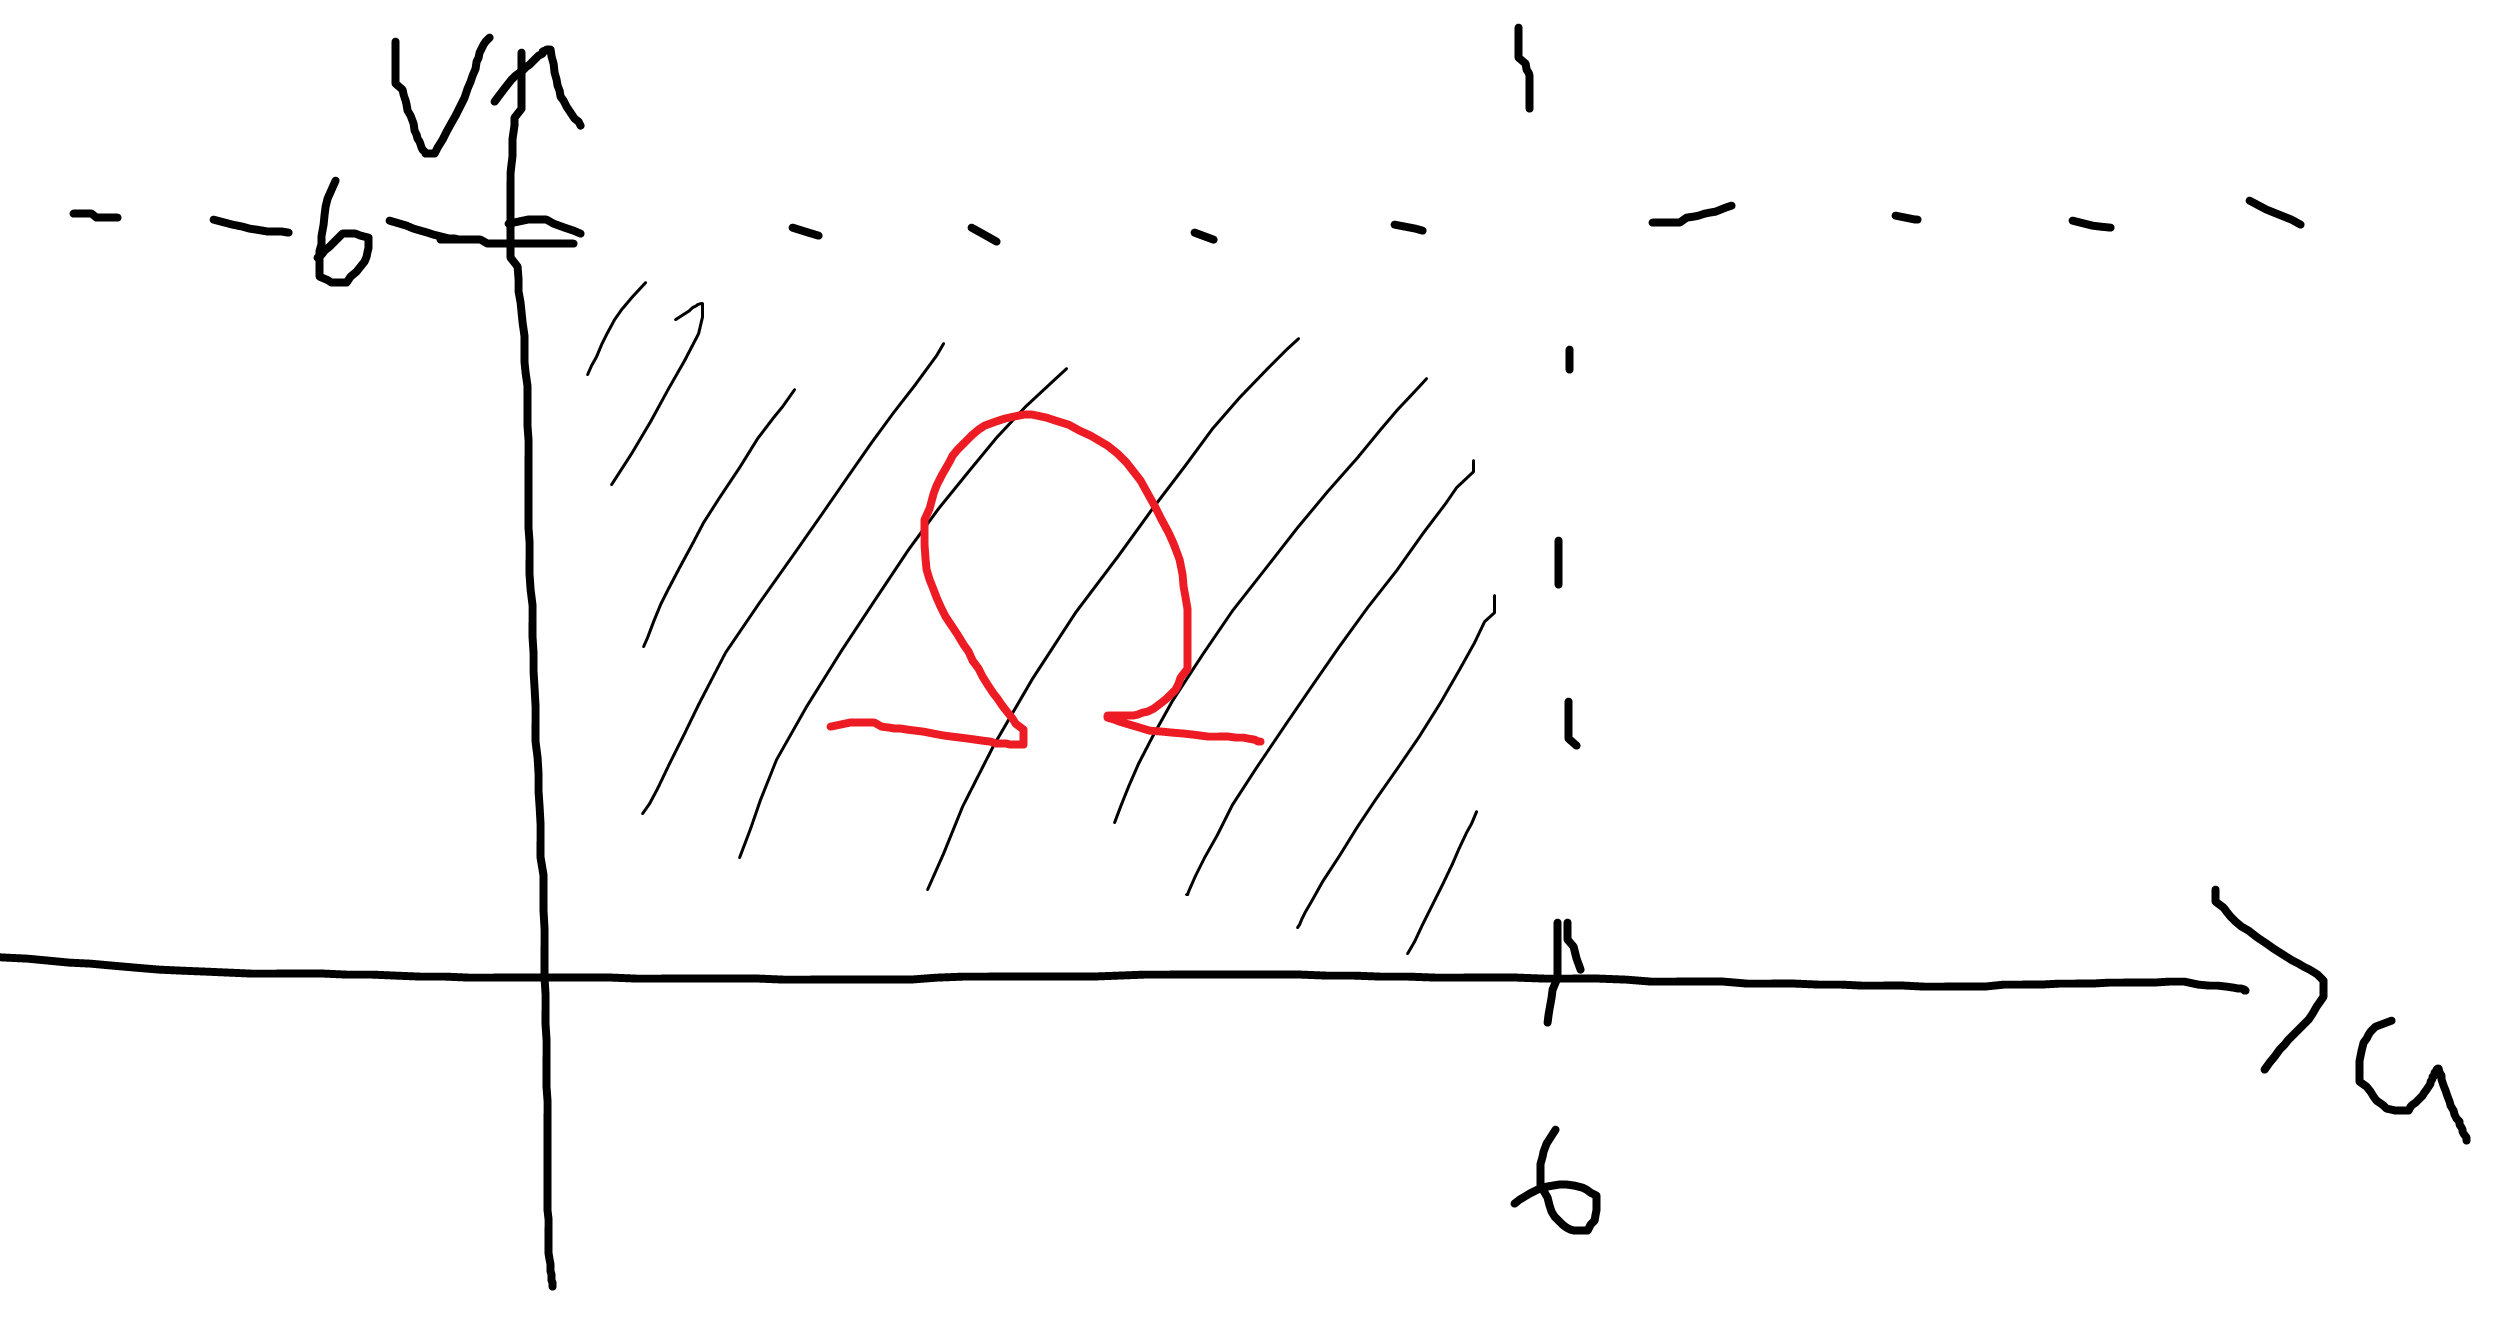
\includegraphics[width=7cm]{kepek/02.png}
			\caption{}
		\end{figure}
		\[ \left.\begin{gathered}
		u+v=2x\\
		u-v=6
		\end{gathered}\right\}\quad \begin{bmatrix}
		x\\y
		\end{bmatrix}=\phi \begin{bmatrix}
		u\\v
		\end{bmatrix}=\begin{bmatrix}
		\frac{u+v}{2}\\\frac{u-v}{6}
		\end{bmatrix},\quad \varOmega=\phi\left([0,6]\times[0,6]\right) \]
		Megoldás (3.):
		\[ \int_{\varOmega}^{}xy\,d(x,y)\overset{\#}{=}\int_{[0,6]\times[0,6]}^{}\frac{u+v}{6}\cdot\frac{u-v}{6}\cdot\frac{1}{6}\,d(u,v)=\frac{1}{72}\int_{0}^{6}\left(\int_0^6(u^2-v^2)\,du\right)\,dv=* \]
		\[ \#: \quad \det[\phi'(u,v)]=\det \begin{bmatrix}
			\frac{1}{2}&\frac{1}{2}\\
			\frac{1}{6}&-\frac{1}{6}
		\end{bmatrix}= \frac{1}{12}-\frac{1}{12}=-\frac{1}{6}\not=0\]
		%when kovács sanyi asks a question and one and a half of minutes awkward silence follows
		\[ *=\frac{1}{72}\int_{0}^{6}\left( \left[\frac{u^3}{3}-uv^2\right]_{u=0}^{u=6} \right)\,dv=\frac{1}{72}\int_0^6\{72-6v^2 \}\,dv=\frac{1}{72}[72v-2v^3]_0^6=0  \]  
		%NOTE id: AnalAlkKS pw: eljenazanalizis
	\end{task}
	\begin{task}
		Legyen
		\[ \varOmega:=\{ (x,y)\in\R^2\ : \ 1\leq x^2+y^2\leq4 \},\quad \int_{\varOmega}^{}\ln(x^2+y^2)\,d(x,y)=? \]
		
		Megoldás: Megállapítható, hogy egy gyűrű az $\varOmega$.
		\begin{figure}[H]
			\centering
			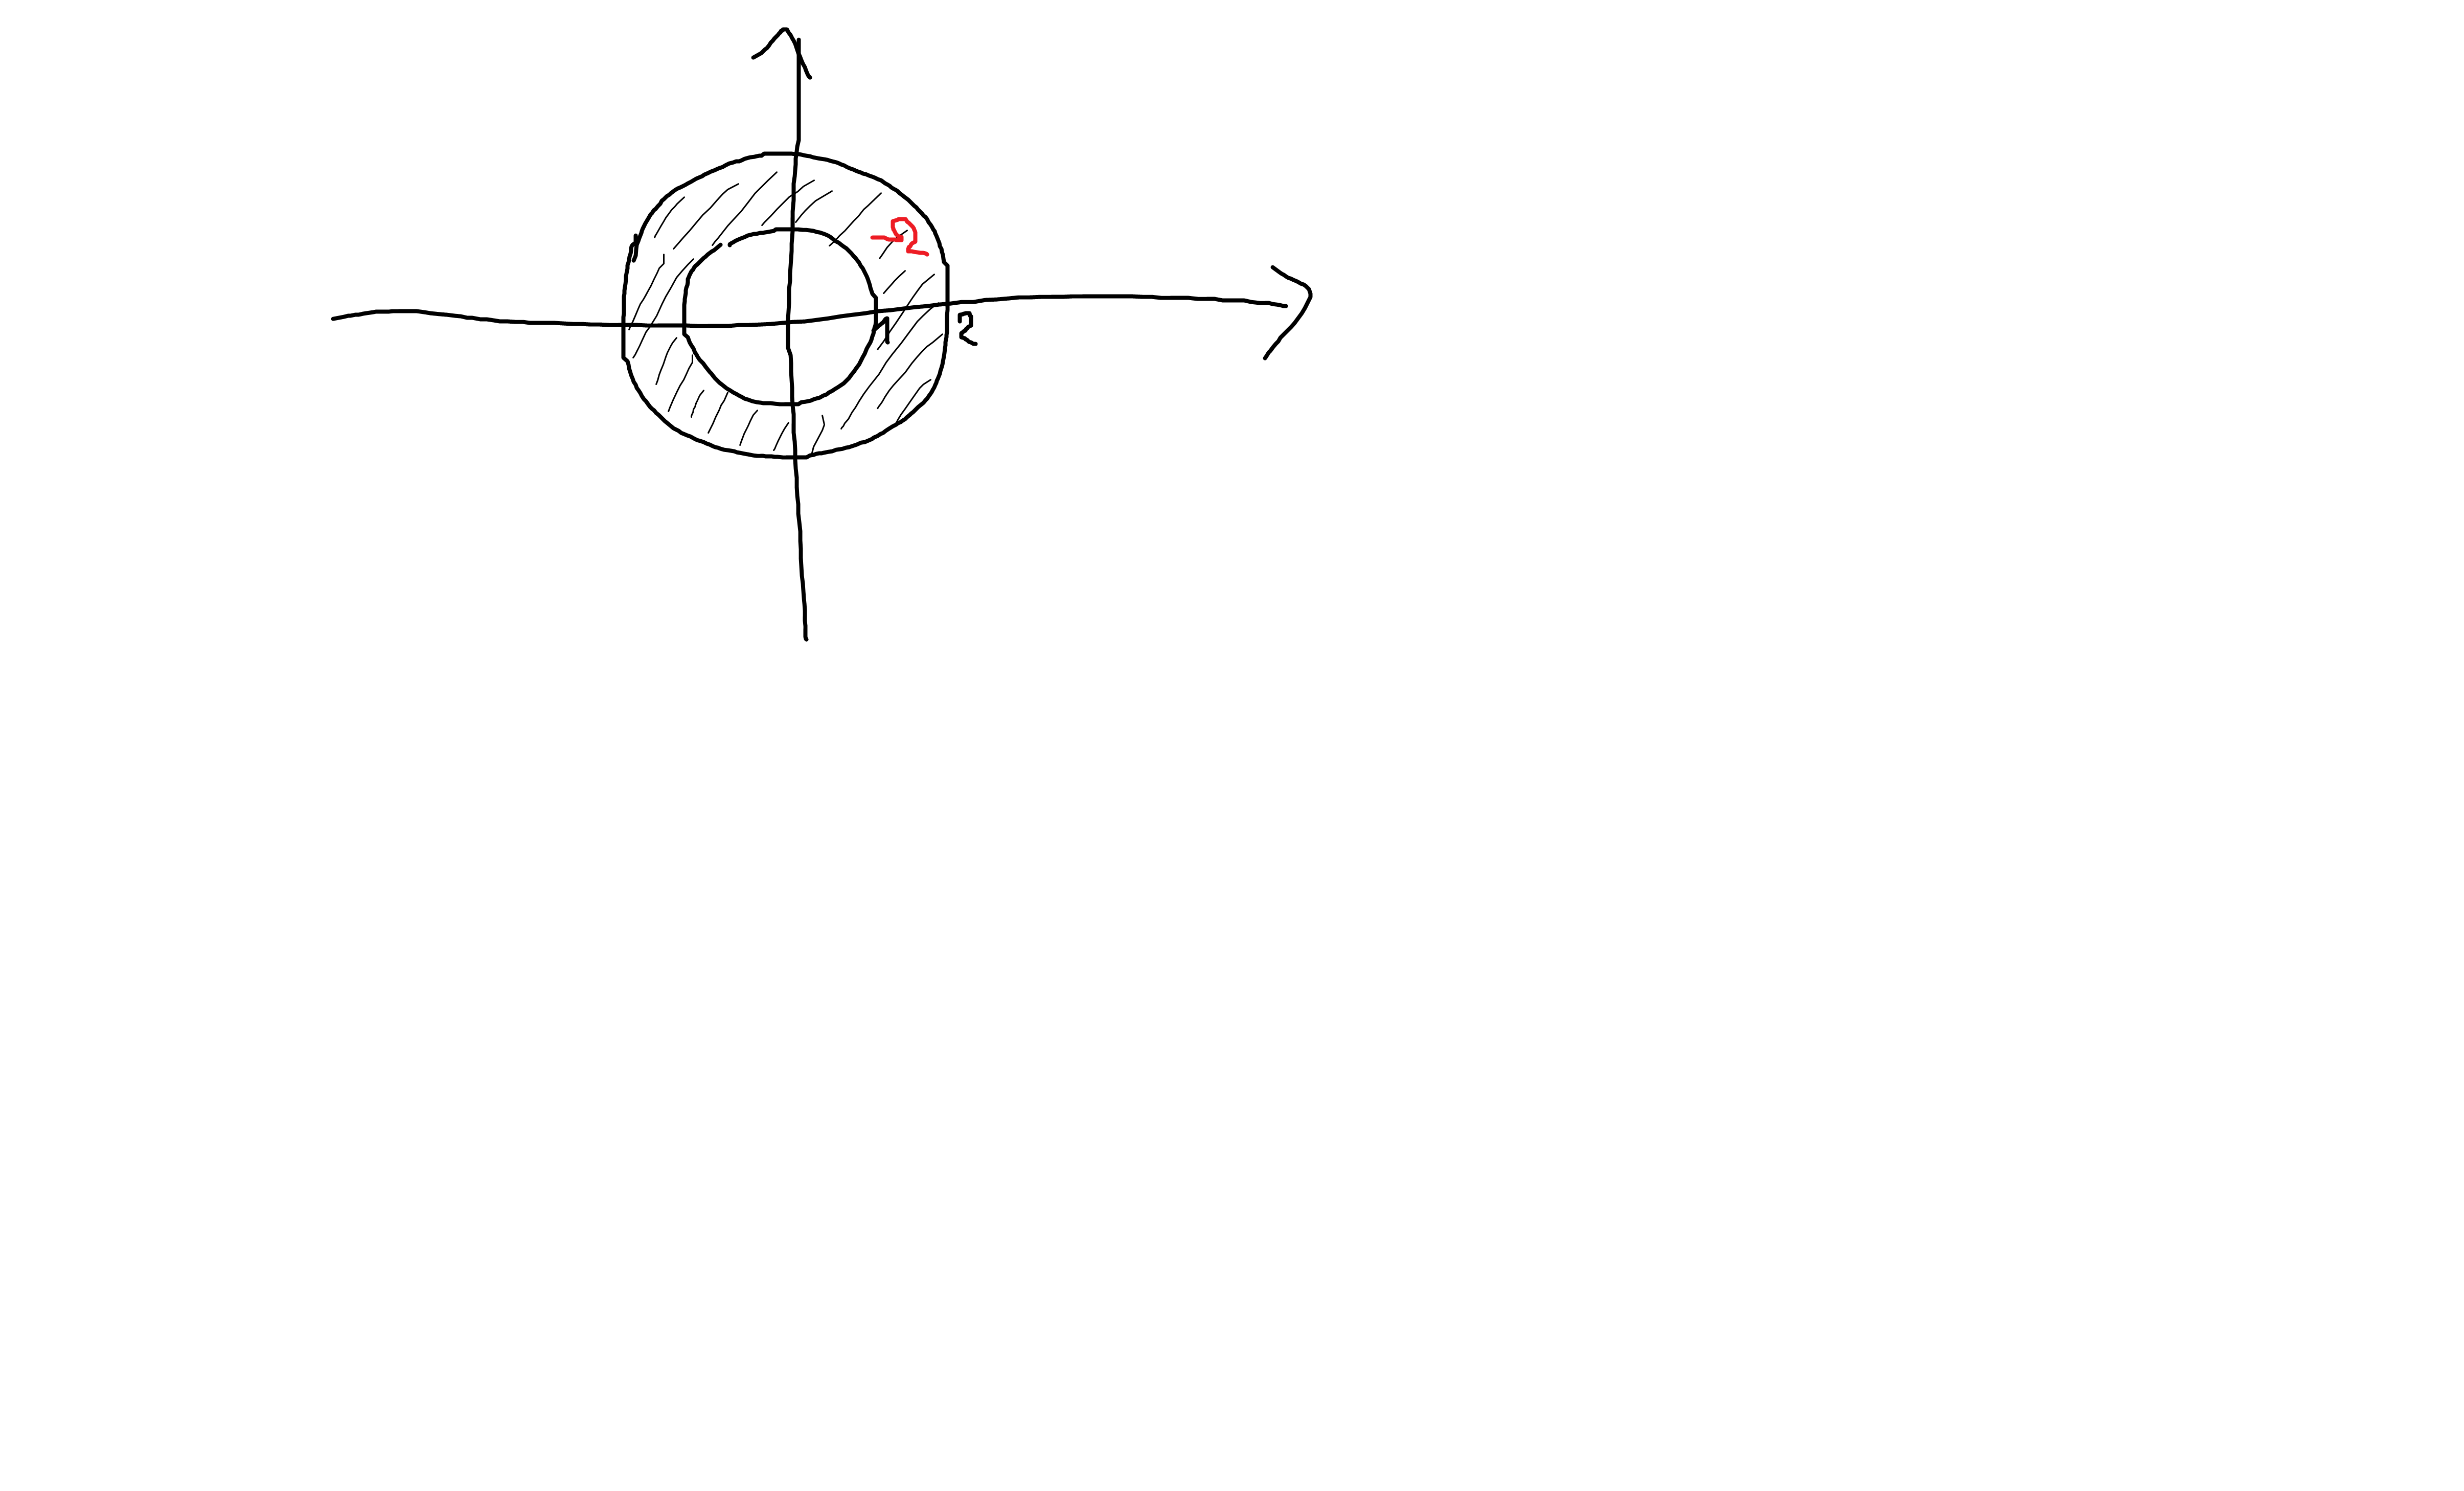
\includegraphics[width=3cm]{kepek/03.png}
			\caption{}
		\end{figure}
		
		\[ \varOmega=\{ \phi(r,v)\in\R\ :\ r\in[1,4],v\in[0,2\pi] \} \]
		\[ \phi(r,v):=\left(r\cos(v),r\sin(v)\right),\quad (r\in(0,+\infty),\ v\in[0,2\pi]) \]
		\[ \det[\phi'(r,v)]=\det \begin{bmatrix}
			\cos(v)&-r\sin(v)\\
			\sin(v)&r\cos(v)
		\end{bmatrix}=r\cos^2(v)+r\sin^2(v)=r\not=0 \]
		\[\Rightarrow\quad \int_{\varOmega}^{}\ln(x^2+y^2)\,d(x,y)=\int_{[1,4]\times[0,2\pi]}^{}\ln(r^2\cos^2(v)+r^2\sin^2(v))r\,d(r,v)=\]
		\[=\int_{0}^{2\pi}\left(\frac{1}{2}\int_{1}^{2}2r\ln(r^2)\,dr\right)\,dv=\frac{1}{2}\int_{0}^{2\pi}\left\{[r^2\ln(r^2)]_1^2-\int_{1}^{2}r^2\cdot\frac{2r}{r^2}\,dr\right\}\,dv=\frac{1}{2}\int_0^{2\pi}\left\{4\ln(4)-[r^2]_1^4 \right\}\,dv=\pi(8\ln(2)-3) \] 
	\end{task}
	\begin{task}
		$a,b>0$
		\[ \varOmega:=\{ (x,y)\in\R^2:\quad \frac{x^2}{a^2}+\frac{y^2}{b^2}\leq1 \} \]
		\begin{figure}[h]
			\centering
			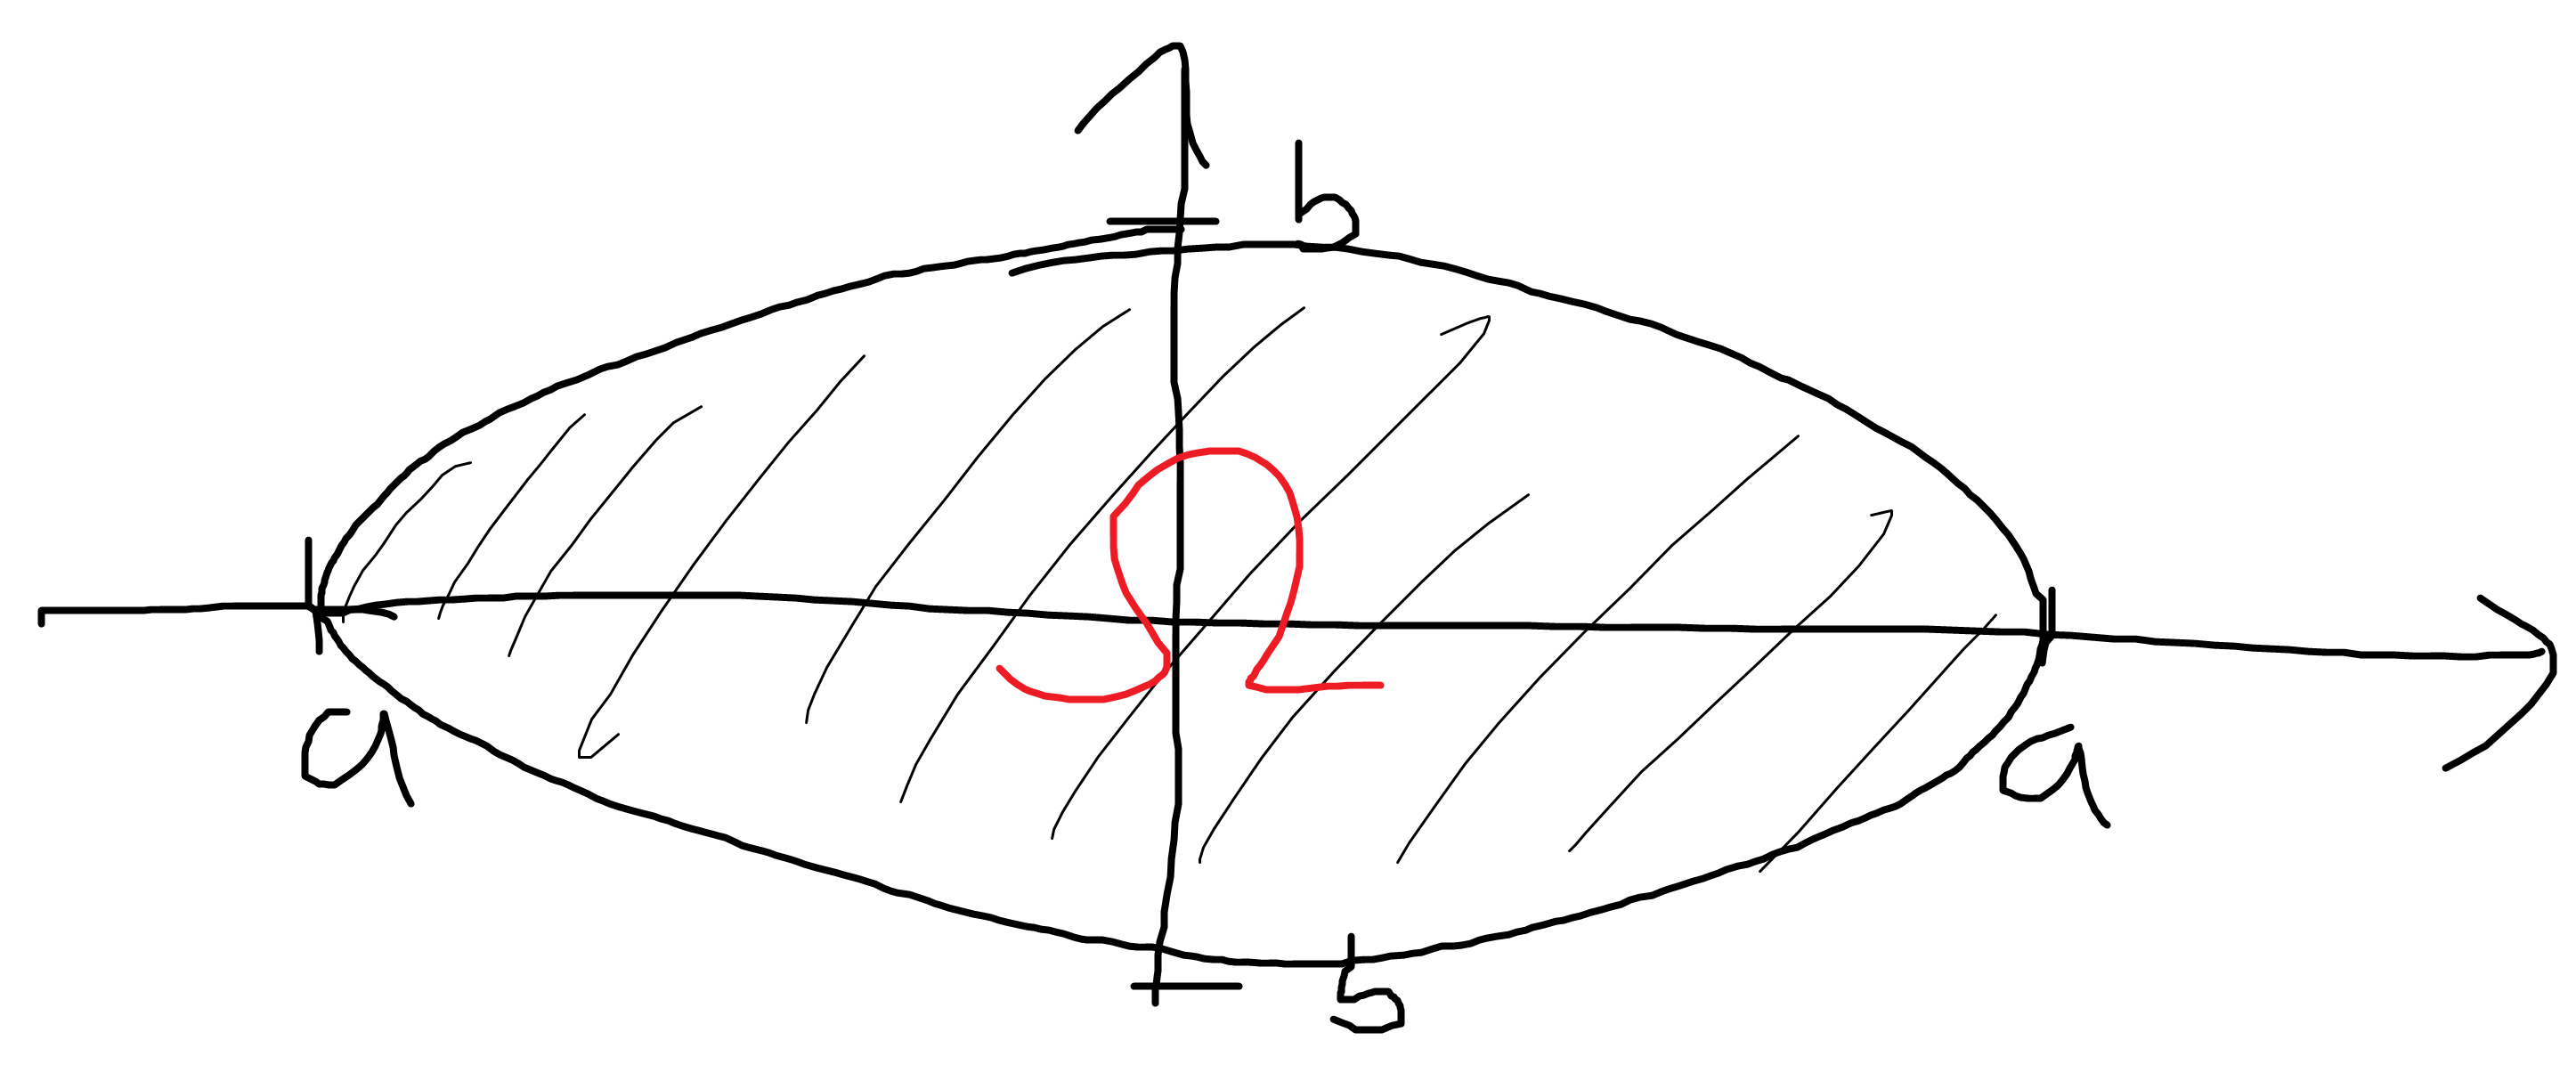
\includegraphics[width=7cm]{kepek/04.png}
			\caption{}
		\end{figure}
		
		Megoldás: $|\varOmega|=?$
		\[ |\varOmega|=\int_{\varOmega}^{}1=* \]
		\[ \varOmega=\{ \phi(r,v)\in\R^2\ : \ r\in[0,1],\ v\in[0,2\pi] \} \]
		\[ \phi:=(ar\cos(v),br\sin(v)) \]
		\[ \det[\phi'(r,v)]=\det \begin{bmatrix}
			a\cos(v)&-br\sin(v)\\
			b\sin(v)&br\cos(v)
		\end{bmatrix}=\ldots=abr\not=0 \]
		\[ *=\int_{[0,1]\times[0,2\pi]}^{}1abr\,d(r,v)=\int_{0}^{2\pi}\left(\int_0^4abr\,dr\right)\,dv=\int_0^{2\pi}\left(ab\left[\frac{r^2}{2}\right]_0^1\right)\,dv=\int_0^{2\pi}\frac{ab}{2}\,dv=ab\pi \]
	\end{task}
	\begin{task}
		\[ R_F=6380km,\quad R_M=1700km,\quad d=60m \]
		\begin{figure}[h]
			\centering
			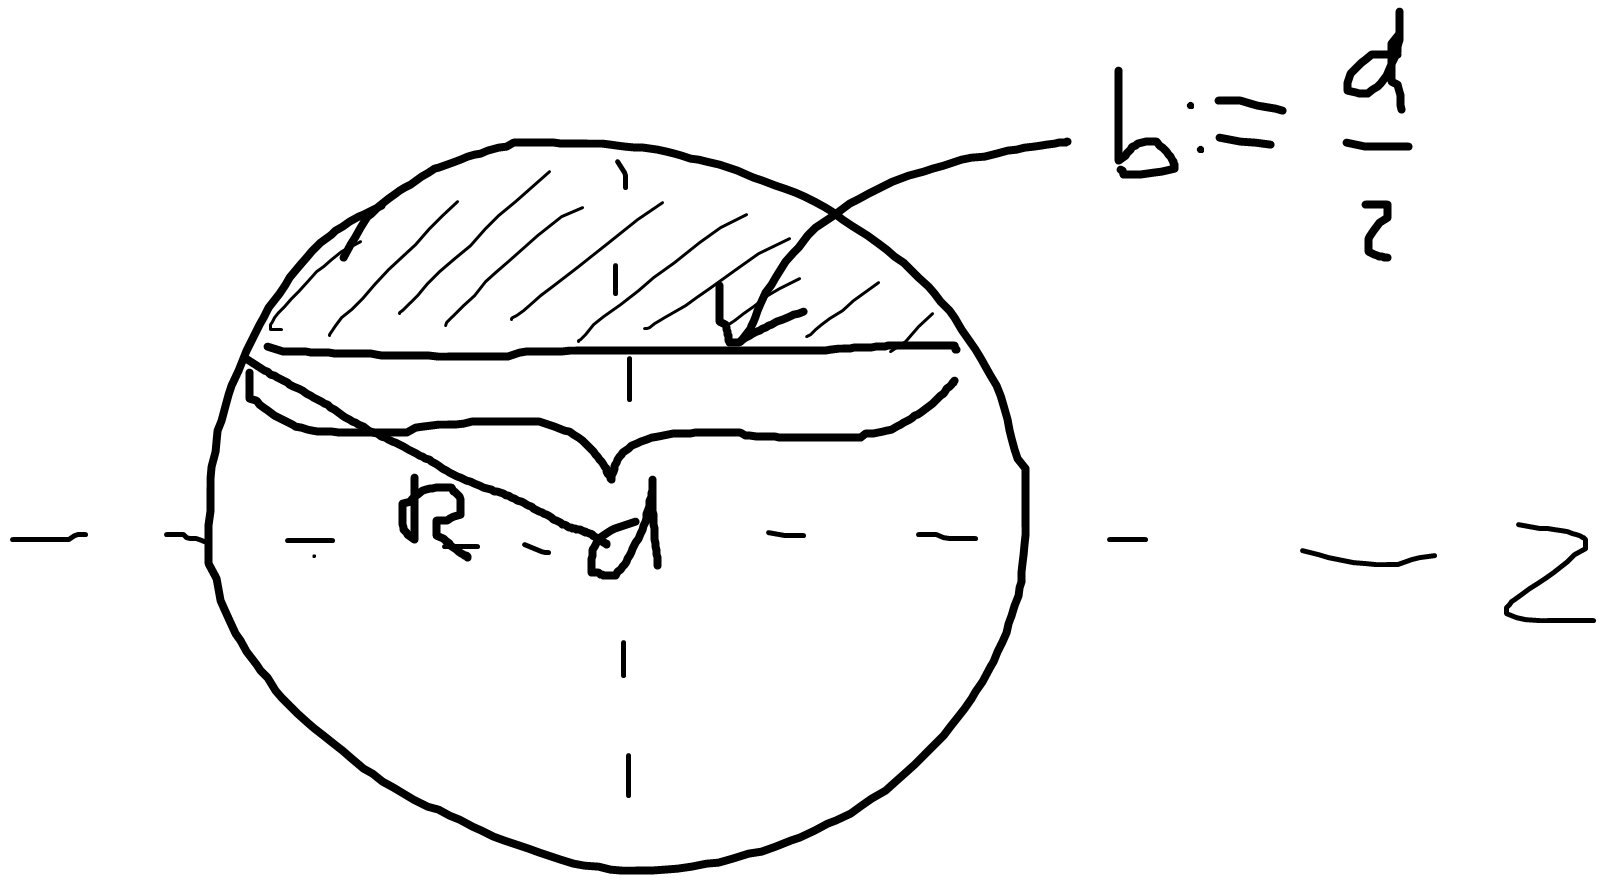
\includegraphics[width=7cm]{kepek/05.png}
			\caption{}
		\end{figure}
		
		Megoldás:
		\[ \phi:=\R^+\times[0,2\pi]\times\R,\quad \phi(r,v,z):=\begin{cases}
			r\cos(v)\\
			r\sin(v)\\
			z
		\end{cases}\]\[ \det[\phi'(r,v,t)]=\det \begin{bmatrix}
			\cos(v)&-r\sin(v)&0\\
			\sin(v)&r\cos(v)&0\\
			0&0&1
		\end{bmatrix}=...=r \]
		\[ |\varOmega|=\int_{\varOmega}^{}1=\int_{-b}^{b}\left(\int_{0}^{2\pi}\left(\int_{\sqrt{R^2-b^2}}^{\sqrt{R^2-z^2}}1r\,dr\right)\,dv\right)\,dz=\int_{-b}^{b}\left(\int_0^{2\pi}\left(\left[\frac{r^2}{2}\right]_{\sqrt{R^2-b^2}}^{\sqrt{R^2-z^2}} \right)\,dv\right)\,dz=\]
		\[=\frac{1}{2}\int_{-b}^{b}\left(\int_{0}^{2\pi}(b^2-z^2)\,dv\right)\,dz=\pi\int_{-b}^{b}(b^2-z^2)\,dz=\pi\int_{-b}^{b}(b^2-z^2)\,dz=\pi\left[b^2z-\frac{z^3}{3}\right]^b{-b}=\]
		\[=\pi\left\{ b^3-\frac{b^3}{3}+b^3-\frac{b^3}{3} \right\}=\frac{4b^3}{3}\pi=\pi\cdot\frac{d^3}{6} \]
	\end{task}
	\subsection{Paraméteres integrál}
	\begin{revision}
		$U\subset\R^d$ nyílt halmaz, $f:U\times[a,b]\to\R,\ f\in C$
		\[ F(r):=\int_{a}^{b}f(r,t)\,dt\quad (r\in U) \]
		Ezt hívjuk paraméteres integrálnak. Tudjuk, hogy $F\in C$, továbbá
		\begin{enumerate}
			\item $f\in C^1\quad \Rightarrow\quad F\in C^1$
			\item $\exists k\in\{1,\ldots,d\}:\quad \partial_k f\in C\quad \Rightarrow\quad \partial_k F\in C$ és 
			\[ \partial_k F(r)=\int_0^b \partial_k f(r,t)\,dt\quad (r\in U) \]
		\end{enumerate}
	\end{revision}
	\begin{example}
		\[ F(x):=\int_1^\pi \frac{\sin(tx)}{t}\,dt\quad (0<x\in\R) \]
		\[ \Rightarrow\quad F'(x)=\int_1^\pi\cos(tx)\,dt,\quad F''(x)=\int_1^\pi -t\sin(tx)\,dt \]
	\end{example}
	\begin{example}
		$$\phi(x):=\int_0^1\ln(x^2+t^2)\,dt\quad (0<x\in\R)\quad \Rightarrow\quad \phi\in C^1$$ és $$\phi'(x)=\int_0^1\frac{\partial}{\partial x}\ln(x^2+t^2)\,dt=\int_0^1\frac{2x}{x^2+t^2}\,dt=\frac{2x}{x^2}\int_0^1\frac{1}{1+\left(\frac{t}{x}\right)^2}\,dt=$$
		$$=\frac{2}{x}\int_0^1\frac{1}{1+\left(\frac{t}{x}\right)^2}\,dt=2\left[\arc\tg\left(\frac{t}{x}\right)\right]_{t=0}^{t=1}=2\arc\tg\left(\frac{1}{x}\right)$$
	\end{example}
	\begin{note}
		$$\phi(x)=\int_0^11\ln(x^2+t^2)\,dt=[t\ln(x^2+t^2)]_{t=0}^{t=1}-\int_0^1t\cdot\frac{2t}{x^2+t^2}\,dt=\ln(x^2+1)-2\int_0^1\frac{t^2}{x^2+t^2}\,dt=$$
		$$=\ln(x^2+1)-2\int_0^1\frac{x^2+t^2-x^2}{x^2+t^2}\,dt=\ln(x^2+1)-2\left\{ 1-\int_0^1\frac{x^2}{x^2+t^2}\,dt \right\}=$$ $$=\ln(x^2+1)-2+2\int_0^1\frac{1}{1+\left(\frac{t}{x}\right)^2}\,dt=\ln(x^2+1)-2+2x\arc\tg\frac{1}{x}\quad (x>0)$$
		$$\Rightarrow\quad \phi'(x)=\frac{2x}{x^2+1}+2\arc\tg\left(\frac{1}{x}\right)+2x\cdot\frac{-\frac{1}{x^2}}{1+\left(\frac{1}{x}\right)^2}=\frac{2x}{x^2+1}+2\arc\tg\left(\frac{1}{x}\right)-\frac{2x}{x^2+1}$$
	\end{note}
	\begin{theorem}
		$U\subset\R$ nyílt halmaz, $f:U\times[a,b]\to\R,\quad f\in C^1,\quad \phi:U\to[a,b],\quad \phi\in D$
		\[ F(x):=\int_a^{\phi(x)}f(x,y)\,dy\quad (x\in U)\quad \Rightarrow\quad F\in D \]
		és
		\[ F'(x)=f(x,\phi(x))\cdot\phi'(x)+\int_a^{\phi(x)}\partial_1 f(x,y)\,dy \]
		
		Bizonyítás: 
		\[ I(t,x):=\int_a^f(x,y) \,dy,\quad G(X):=(\phi(x),x),\quad (t\in[a,b],\ x\in U) \]
		$ \Rightarrow\quad F=I\circ G\in D,\quad \text{ui.}\quad I\in D, G\in D$, így
		\[ F'(x):=\langle (I'\circ G)(x),G'(x)\rangle=* \]
		\[ G'(x)=(\phi'(x),1),\quad I'(t,x)=(\partial_1I(t,x),\partial_2I(t,x))=(f(x,y),\int_a^1\partial_1f\left(x,y\,dy\right) \]
		\[ *=f(x,\phi(x))\cdot \phi'(x)+\int_0^{\phi(x)}\partial_1f(x,y)\,dy\cdot1 \]
	\end{theorem}
	\begin{note}
		$U\subset\R$ nyílt, $\phi, \psi:U\to[a,b]:\quad \phi\leq\psi,\quad f:U\times[a,b]\to\R,\quad f\in C^1$.
		\[ F(x)=\int_{\phi(x)}^{\psi(x)}f(x,y)\,dy\quad (x\in U)\quad \Rightarrow F'(x)=f(x,\psi(x))\cdot\psi'(x)-f(x,\psi(x))\cdot\phi'(x)+\int_{\phi(x)}^{\psi(x)}\partial_1f(x,y)\,dy \]
	\end{note}
	\begin{example}
		$f:\R\to\R,\quad f\in C^1,\quad F(x):=3f(x)+2xf'(x)\quad (x\in\R)$
		\[ \Rightarrow\quad F\in D^2\quad \text{és}\quad F''(x)=3f(x)+2xf'(x)\quad (x\in\R) \]
		$h(x,y):=(x+y)f(y)\quad ((x,y)\in\R^2)\quad \Rightarrow\quad h\in C^1\quad \Rightarrow\quad F\in D$ és
		\[ F'(x)=\underbrace{2x\cdot f(x)}_{h(x,x)}\cdot1+\int_0^x\partial_1h(x,y)\,dy=2xf(x)+\int_0^xf(y)\,dy \]
		$f\in D\quad \Rightarrow\quad F'\in D$ és 
		\[ F''(x)=2f(x)+2xf'(x)+f(x)=3f(x)+2xf'(x) \]   
	\end{example}
\end{document}